%% Erläuterungen zu den Befehlen erfolgen unter
%% diesem Beispiel.

\documentclass{scrartcl}

\usepackage[utf8]{inputenc}
\usepackage[T1]{fontenc}
\usepackage{lmodern}
\usepackage[ngerman]{babel}
\usepackage{amsmath}
\usepackage{graphicx}
\usepackage{tikz}
\usepackage{fancyhdr} %Header
\usepackage{libertine}

\usetikzlibrary{automata,positioning}

\title{Verteiltes Genom Browsing}
\subtitle{Grobspezifikation}
\author{Malte Kruse, Ben Schumacher}

\setkomafont{subtitle}{\bfseries \LARGE}
\renewcommand{\headrulewidth}{0pt}
%\date{6. September 2015}
\begin{document}
\pagestyle{fancy}
%\fancyhf{}
\cfoot{}
\rfoot{\pagemark}
\lhead{}
\rhead{}
%\textbf{Logik in der Informatik}}
%\hfill
%\section*{Projektplan}

\setcounter{page}{-1}
\maketitle
\thispagestyle{empty}

\newpage
\tableofcontents
\thispagestyle{empty}

\newpage
\section{Einleitung}

Dies ist die Grobspezifikation für das Semesterprojekt zur verteilten Echtzeitrecherche in Genomdaten. 
Hierbei umfasst der Begriff "'Genomdaten"':
\begin{description}
\item[Chromosomen] enthalten das Erbgut eines Menschen. Sie enthalten somit die DNA, auf welcher die einzelnen Gene abgebildet sind. Verschiedene Lebewesen haben unterschiedlich viele Chromosomen und Gene. 
\\ Für dieses Projekt beziehen wir uns ausschließlich auf die 24 Chromosomen des Menschen. Hier sind die zwei Geschlechtschromosomen X und Y bereits enthalten.

\item[Gene] bestehen aus einer Sequenz von Basen, welche ein zu synthetisierendes Protein kodieren. Jedes Gen kodiert genau ein Protein. Jedes Gen kann auf Grund seiner Genkoordinaten gefunden werden.

\item[Genkoordinaten] geben an, auf welchem Abschnitt des Chromosoms ein Gen liegt.
Hierbei werden die untere und die obere Grenze angegeben.

\item[Basenpaare] ergeben sich durch die Doppelhelix-Struktur der DNA.\\ Es gibt vier Basen:
\begin{enumerate}
\item Adenin (A) 
\item Cytosin (C)
\item Guanin (G)
\item Thymin (T)
\end{enumerate}
 von denen jeweils zwei Gegenstücke zueinander sind. Diese Paare sind A - T und C - G. Es folgt also, dass nur diese Basenpaare in der Helix vorhanden sind.\\
Spricht man von MBp, so sind dies Megabasenpaare, hierbei entspricht\\
1Mbp = 1000000 Bp (Basenpaare).

\item[Mutationen] sind Abweichungen in der Basensequenz eines Gens zum Referenzgenom. Das heißt:\\Unterscheidet sich an einer spezifischen Stelle des Gens eines Probanden eine Base zu der im Referenzgenom verzeichneten, so ist dies eine Punktmutation.

\item[Das Referenzgenom] wird alle drei Monate, also einmal pro Quartal, neu festgelegt. An Hand dieses Genoms werden alle weiteren Sequenzierungen von Basenpaaren überprüft und Mutationen ermittelt. 
\end{description}
Im folgenden Dokument wird die genaue Aufgabenstellung sowie deren Umsetzung erläutert.

\newpage
\section{Aufgabenstellung und Anforderungen}
\subsection{Aufgabenstellung}
Es soll ein System entwickelt werden, welches in Echtzeit Genomdaten durchsucht und die grafische Auswertung übernimmt. 
\subsection{Anforderungen}
\begin{itemize}

\item Es werden vier Datenbanken fest integriert: 
\begin{itemize}
\item HGMD\footnote{\label{foot:1}http://www.hgmd.cf.ac.uk/ac/index.php}
\item dbSNP\footnote{\label{foot:2}http://www.ncbi.nlm.nih.gov/SNP/}
\item 1000 Genomes Project\footnote{\label{foot:3}http://www.1000genomes.org/}
\item The Cancer Genome Atlas: Lung and Colorectal Cancer\footnote{\label{foot:4}http://cancergenome.nih.gov/}
\end{itemize}
Weiterhin wird das System für weitere (eigene) Datenquellen erweiterbar sein.

\item Folgende Informationen werden bereitgestellt:
\begin{itemize}
\item Metadaten: Datenquelle, Zeitpunkt des Downloads
\item Genkoordinate der Mutation (ggf. Abschnitt)
\item Mutierte Basensequenz (auch Referenzgenom muss bekannt sein)
\item (relative) Häufigkeit der Mutationen
\item Quellspezifische Sample-Attribute (Krankheit, Geschlecht, etc.)
\end{itemize}

\item Eine Anfrage wird in <1 Sekunde durchlaufen.\\
Zulässige Anfragen sind:
\begin{itemize}
\item Intervallanfragen:
\begin{itemize}
\item Anfrage mit: Chromosom, linke und rechte Grenze (Genkoordinaten)
\item Systemkorrektur: Intervall >10Mbp verkleinern auf 10Mbp
\item Ergebnis: Anzahl der Mutationen in dem Abschnitt
\end{itemize}
\item Genanfragen:
\begin{itemize}
\item Anfrage mit: Name eines humanen Gens
\item Systemkorrektur: Namensvorschläge, wenn Genname nicht vollständig bekannt
\item Ergebnis: Vom System bestimmter Genabschnitt
\end{itemize} 
\end{itemize}
\newpage
Folgende Filter werden zur Suchoptimierung angeboten:
\begin{itemize}
\item Einschänkung auf Quelle
\item Einschänkung auf relative Häufigkeit
\item Gleichheit quellspezifischer Attribute
\end{itemize}

\item Die Darstellung erfolgt:
\begin{itemize}
\item je Datenquelle
\item mit einem max 10Mbp großen Ausschnitt des Chromosoms
\item mit Referenzgenom zum Vergleich bei kleinen Abschnitten
\item mit Anzeige der Basenpaare und Markierung von Mutationen in kleinen Abschnitten ($\leq$ 200Bp)
\item mit Andeutung der Verteilung der Häufigkeit von Mutationen in großen Abschnitten (> 200Bp)
\end{itemize}
Zudem bietet das Interface interaktiv Möglichkeiten:
\begin{itemize}
\item Zoomfunktion, um den dargestellten Bereich zu verkleinern oder zu vergrößern
\item Srcollen, um sich horizontal auf dem Gen fortzubewegen
\item Konfigurationsmöglichkeiten zur Darstellung und anderer Systembereiche
\end{itemize}

\item Das System wird unter Mozilla Firefox laufen und auf bestehenden Webservern leicht einzurichten sein
\end{itemize}

\newpage
\section{Beispiele zur Nutzung: Use Cases}
\subsection{Use Case 1}
Ein Benutzer möchte herausfinden, welche Mutationen im Bereich von 144MB – 154MB auf dem Chromosom 7 auftreten können. Hierfür wählt er die 1000 Genomes Projekt-Datenbank aus. \\
Das ganze Chromosom in einem eigenen Anzeigebereich (Lane) im Vergleich zum Referenzgenom angezeigt. Er erkennt durch eine Markierung, dass im Bereich von 150MB-152MB gehäuft Mutationen auftreten können. Da er diesen Bereich nicht detailliert einsehen kann, zoomt der Benutzer herein. Die Basenpaare, sowohl in der 1000 Genomes-Lane als auch vom Referenzgenom, sind immer detaillierter zu erkennen, bis er genau einsehen kann, welche Mutationen auftreten können. Bei erreichen der maximale Zoomstufe, sind alle Basenpaare des Chromosoms 7 und des Referenzgenoms zu erkennen und er kann die auftretenden Mutationen betrachten.
\subsection{Use Case 2}
Ein Benutzer möchte herausfinden, welche Mutationen bei einer bestimmten relativen Häufigkeit im Bereich eines Gens auftreten. Da er sich sehr für den colorectalen Bereich interessiert, wählt er The Cancer Genome Atlas (TCGA) aus. Da der Benutzer nicht den genauen Namen des Gens kennt und sich bei der Eingabe irrt, bekommt er keine Basenpaare angezeigt, sondern Vorschläge, welches Gen er gesucht haben könnte. Auf Grund der Vorschläge erinnert sich der Benutzer und wählt das korrekte Gen. \\
Es erscheint eine Lane, welche die Daten für den Bereich darstellt und der Benutzer erkennt die Bereiche, in welchen Mutationen auftreten. Zusätzlich werden ihm die relativen Häufigkeiten der Mutationen angezeigt.
\subsection{Use Case 3}
Ein Benutzer möchte sich darüber informieren, mit welcher Häufigkeit in einem bestimmten Bereich eines bestimmten Gens Mutationen auftreten können. Hierbei wählt er die HGMD mit einem Bereich von 140MB – 155MB. Da der Bereich jedoch zu groß ist,
wird ihm nur der Bereich von 140MB-150MB dargestellt. \\
Er erkennt in diesem Bereich, dass sehr wenig Mutationen auftreten. Ihn interessiert jedoch ebenfalls, ob bei Krebspatienten höhere Mutationsraten existieren. Dazu führt er die gleiche Suche noch einmal aus, wählt jedoch zusätzlich TCGA für Lungenkrebs und TCGA für Colorectalkrebs. \\
Als Ergebnis werden ihm die drei Lanes untereinander angezeigt und er kann die Häufigkeit von Mutationen in den Bereichen vergleichen.

\newpage
\section{Umsetzung}
\subsection{Vorgehensweise des Systems}
Damit dem System Daten zur Verfügung stehen, müssen die vier Hauptdatenbanken bei Programmstart zuerst aus dem Internet heruntergeladen werden.\\
Nachdem der Download erfolgreich war, werden die Datenbanken in ein einheitliches Format überführt. Ist die Vereinheitlichung vollzogen, können nun die humanen Datensätze herausgefiltert und in das Datawarehouse (DWH) eingespeichert werden.
\\
Sind alle Daten verarbeitet und somit das DWH vollständig, stehen die Daten zum Aufbau des verteilten Index zur Verfügung. \\
Wurde der verteilte Index fertig gebaut, kann der Benutzer nun Anfragen an das System absenden. Die Anfragen werden vom Userinterface (GUI) an die Middleware geschickt. Hier werden die Anfragen validiert und gegebenenfalls korrigiert. Sind die Anfragen korrekt, werden diese über den verteilten Index ausgeführt und die Ergebnisse an das GUI zurückgegeben. Hat das GUI die Ergebnisdaten empfangen, werden diese grafisch aufbereitet. Nun werden die vom Benutzer angefragten Informationen grafisch dargestellt.\\\\
Folgendes Kommunikationsdiagramm verdeutlicht hierbei den Ablauf:\\\\
\begin{center}
\begin{tikzpicture}[%
>=stealth,
node distance=5cm,
on grid,
draw,
align=left
]
\node[rectangle, draw, initial,initial text=] (0) {Download\\der Datensätze};
\node[rectangle, draw] (1) [right=3cm of 0] {Parsing};
\node[rectangle, draw] (2) [right=3cm of 1] {Einfügen\\in DHW};
\node[rectangle, draw] (3) [below=2cm of 0] {Aufbau der \\Index Bäume};
\node[rectangle, draw] (4) [right of=3] {Suchoperationen in den\\Bäumen ausführen};
\node[rectangle, draw] (5) [below=2cm of 3] {Daten darstellen};
\path[->] (0) edge node {} (1);
\path[->] (1) edge node {} (2);
\path[->] (2) edge node {} (3);
\path[->] (3) edge node {} (4);
\path[<->,bend left, left] (4) edge node {JSON} (5);
\end{tikzpicture}
\end{center}
\subsection{Arbeitsbreiche}
Zur Umsetzung des Systems müssen, wie aus \textit{4.1 Vorgehensweise des Systems} hervorgeht, drei Hauptbereiche abgedeckt werden. Diese sind:
\begin{description}
\item[Integration:] Zuständigkeitsbereiche der Integration sind die Aufbereitung der Datenquellen und die Bereitstellung der aufbereiteten Datensätze in einer eigens entworfenen Datenbank.

\item[Middleware:] Die Middleware ist für die Kommunikation zwischen Datenbank und Frontend zuständig. Um die vom Frontend an die Middleware gesendeten Anfragen effizient bearbeiten zu können, befasst sich die Middleware mit dem Entwurf eines verteilten Index. Dieser ermöglicht die zeiteffiziente Suche in den Daten der Datenbank und somit eine zeiteffiziente Rückgabe der Ergebnisse an das GUI.

\item[Frontend:] Das Frontend ist für die grafische Aufbereitung der Ergebnisdaten, sowie für das GUI zur Bedienung des Systems zuständig.
\end{description}
Im folgenden werden die Teilbereiche, die Grundzüge ihrer Realisierung, sowie die zu Verwendung findenden Technologien erläutert. Des Weiteren werden offene Fragen und Risiken der einzelnen Realisierungen angesprochen.

\newpage
\section{Integration}
\subsection{Aufgabe und Systemarchitektur}
\subsubsection{Aufgabe}
Die Integration stellt das DWH zur Verfügung. Hierzu müssen zuerst die zu integrierenden Datenbanken aus dem Internet heruntergeladen werden. Danach erfolgt eine Aufbereitung der Daten in ein einheitliches Format.
Ist dies geschehen, werden die Datensätze über einen Parser in das DWH eingespeichert.
\\
\\ Bevor jedoch diese Schritte realisiert werden können, muss sich die Integration mit der manuellen Analyse der Datensätze beschäftigen. Hieraus ergibt sich ein Datenbankschema, in das alle zu integrierenden Datenbanken überführt werden müssen.
\subsubsection{Architektur}
Die Realisierung erfolgt durch materialisierte Integration in drei Schritten:
\begin{enumerate}
\item Zuerst werden die Datenbanken heruntergeladen und die Datensätze vereinheitlicht.
\item Nachdem dies erfolgt ist, läuft über alle Datensätze ein Parser, der die benötigten Informationen und Metadaten herausliest und in unser Datensatzformat überführt.
\item Die Datensätze werden in das DWH geschrieben.
\end{enumerate}
\subsubsection{Technologien}
Der Download, sowie der Parser werden voraussichtlich in Java realisiert.\\
Für die Datenbank wird verwendet.
\subsection{Risikoanalyse}
Wird ein ungeeignetes DWH entworfen, das bedeutet die ungeeignet Datenbankmanagementsoftware oder ein unpassendes Datenbankschema verwendet, kann dies zu vielen Problematiken führen. Hierunter versteht man unter anderem zeiteffiziente Zugriffsprobleme, sowie mangelnde Erweiterbarkeit des System oder ähnliche Probleme.\\
Um dieses Risiko zu vermeiden, werden die Datensätze sorgfältig analysiert und eine geeigneter erster DWH-Entwurf erstellt. Der Entwurf wird ebenfalls sorgfältig überprüft und bei Problemen verändert. Ist der endgültige Entwurf fertig, wird die Datenbank umgesetzt.\\\\
Es besteht ebenfalls das Risiko, dass neue Datenquellen nur schwer oder falsch eingebunden werden können. Diesem versuchen wir entgegen zu wirken, indem wir einen allgemeinen, modifizierbaren Parser entwickeln wollen, der über die Datensätze läuft. Außerdem wird die Integration neuer Datenquellen möglichst einfach gehalten und gut dokumentiert werden.\\\\
Weiterhin können Probleme mit der Speicherplatzkapazität entstehen. Da noch keine genauen Datengrößen bekannt sind, ist dieses Risiko noch nicht einzuschätzen.\\
Sollte dieser Fall eintreten, muss abgeschätzt werden, wie wir damit umgehen können.
\\\\
Es besteht das Risiko, dass die Datenbanken unterschiedliche Referenzgenome verwenden. In diesem Fall ist unklar, wie damit umgegangen wird.
\subsection{Offene Fragen}
\begin{itemize}
\item TCGA stellt für Projekte ohne Forschungszweck nur Metadaten zur Verfügung, keine Genomdaten. Gibt es eine Alternative oder kann die Bioinformatik "'Forschungszwecke"' geltend machen?
\footnote{\label{foot:5}Seite 12: http://cancergenome.nih.gov/PublishedContent/Files/pdfs/TCGA
\\ \%20Human\%20Subjects\%20Protection\%20and\%20Data\%20Access\%20Policies \\ \%20Rev\_2014-01-16.pdf}
\item Wie sollen verfahren werden, wenn unterschiedliche Referenzgenome verwendet werden?
\end{itemize}
\subsection{Schnittstellen}
Die Schnitstelle zur Middleware wird eine Datenbank darstellen, welche die Daten zur weiteren Verwendung bereitstellt.

\newpage
\section{Middleware}
\subsection{Aufgabe und Systemarchitektur}
\subsubsection{Aufgabe}
Die Aufgabe der Middleware umfasst den Entwurf eines verteilten Index, sowie der Suche auf der Datenbank.\\
Die Daten müssen also aus der Datenbank geladen werden und ein verteilter Index aufgebaut werden. Dieser Index soll hierbei eine zeiteffiziente Suchstruktur darstellen, die in Echtzeit die Datensätze durchsucht. \\Des Weiteren nimmt die Middleware die Anfragen des Benutzers aus dem Frontend entgegen.
Wurde eine Suchanfrage beendet, gibt die Middleware die gefundenen Datensätze an das Frontend zurück.
\subsubsection{Architektur}
Der verteilte Index baut für jede Datenbank einen eigenständigen Intervalltree auf. Ist dies geschehen, werden diese jeweils vollständig auf die vier VMs verteilt.\\
Ist dies geschehen, kann das Frontend Anfragen an die Middleware senden. Diese werden nun über die entsprechenden Intervalltrees abgearbeitet und eine Ergebnisliste wird berechnet. Hierbei werden zunächst nur die angefragten Informationen berücksichtigt. Diese Ergebnisliste wird dann in Form von JSON-Objekten an das Frontend zurückgegeben. \\
Nachdem diese Ergebnisse bereitgestellt wurden, wird die Middleware weitere, wahrscheinlich demnächst benötigte, Informationen vorberechnen und zwischenspeichern. Dazu gehören unter anderem weitere Zoomstufen. Hierdurch soll eine bessere zeiteffizienz bei Anfragen gewährleistet werden, sollten diese angefordert werden.
\subsubsection{Technologien}
Für den verteilten Index wird Java verwendet werden. Die Laufzeitumgebung der Middleware wird ein Tomcat-Server darstellen.
\subsection{Risikoanalyse}
Sollte nur ein Teil der Quellen angefragt werden, sind nicht alle VMs in Benutzung, sondern nur diese, deren Intervalltrees benötigt werden. Damit auch hier ein verteiler Ansatz besteht, wird dementsprechend eine Ergebnisliste erstellt, welche hinterher auf alle VMs aufgeteilt wird, bevor weitere Filter angewandt werden.\\\\
Weiterhin besteht ein Risiko bei der Größe der Intervalltrees. Sind diese zu groß, können unter Umständen nicht alle Daten vorgehalten werden und es muss auf der Datenbank selbst gearbeitet werden. Dies wirkt sich negativ auf die Zeiteffizienz von Suchanfragen aus.\\
Diese Problematik soll dahingehend Umgangen werden, in dem gut durchdachte Intervalltrees aufgebaut werden. Sollte die Datenbank nicht komplett geladen werden können, muss sich eine Swappingmethode überlegt werden.
\subsection{Offene Fragen}
\begin{itemize}
\item Wie werden Genpositionen dargestellt (Stelle, Intervall)?
\item Sollen auch Basensequenzen dargestellt werden oder nur positionelle Daten?
\end{itemize}
\subsection{Schnittstellen}
Die Middleware stellt eine Schnittstelle zur Verfügung, welche es dem Frontend ermöglicht, Anfragen an die Middleware zu senden. Über diese Schnittstelle werden hinterher JSON-Objekte an das Frontend zurückgegeben.

\newpage
\section{Frontend}
\subsection{Aufgabe und Systemarchitektur}
\subsubsection{Aufgabe}
Das Frontend nimmt die Daten der Middleware entgegen und bereitet diese grafisch auf.\\
Neben der Darstellung der Daten ist sie auch für die Konfiguration und die Bedienung des Systems durch den Benutzer zuständig.
\subsubsection{Architektur}
Die Architektur der GUI lässt sich an folgenden Mock-Ups verdeutlichen, welche nur der Anschauung dienen:\\\\
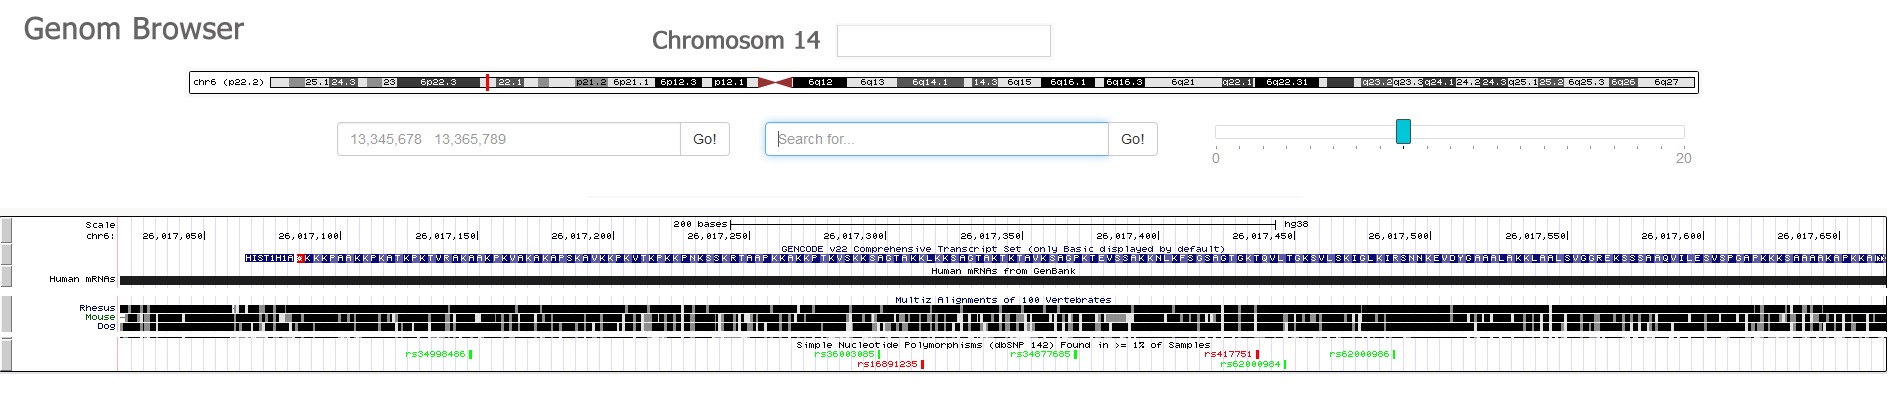
\includegraphics[width=1.0\textwidth]{../mockups/gb_mockup_vereinfacht.png}
Dieses Mock-Up stellt eine vereinfachte Ansicht der Genomdaten dar. Diese wird bei niedrigeren Zoomstufen dargestellt. \\ Oben zu sehen ist das gerade dargestellte Chromosom mit seinen Banden. Hierbei stellt die rote Markierung die Position dar, an der man sich gerade befindet.\\
Unter der Chromosomdarstellung befinden sich die Elemente zur Benutzersuche. Links zu sehen ist das Suchfenster für Intervalle und Genkoordinaten, in der Mitte das für Gene und rechts befindet sich der Zoomstufenregler.\\
Im unteren Bereich des Bildes sind die einzelnen Lanes zu erkennen. Oben befindet sich das Referenzgenom. Darunter sind die Ergebnisse der Suchanfragen an die verschiedenen Datenbanken zu erkennen. Hierbei stellen die Markierungen die Positionen der Mutationen dar.\\\\
Wenn näher herangezoomt wird, sind ab einem gewissen Punkt detailiertere Genabschnitte zu sehen. Folgendes Mock-Up verdeutlicht dies:\\\\
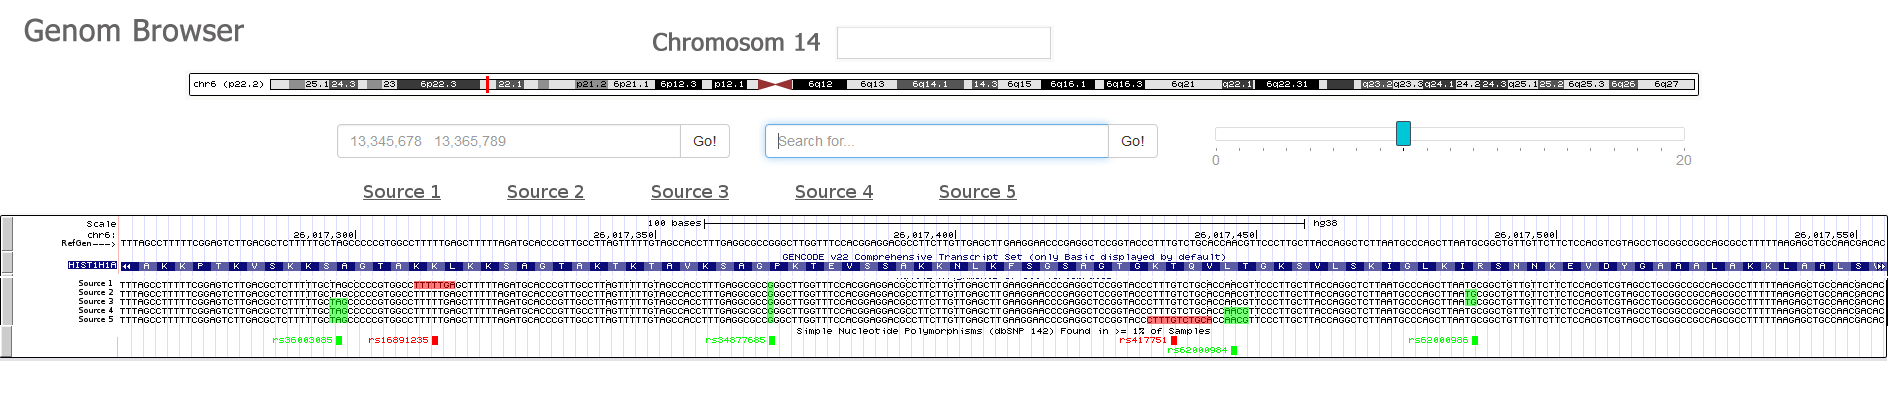
\includegraphics[width=1.0\textwidth]{../mockups/gb_mockup_detail.png}
Es sind nun die einzelnen Basen erkennbar, sowie die Mutationen im Detail ersichtlich.
\subsubsection{Technologien}
Für die Realisierung des Frontends werden XHTML, CSS und JavaScript verwendet. Eine Verwendung von PHP ist nicht ausgeschlossen.\\
Weiterhin werden folgende JavaScript-Bibliotheken benutzt:
\begin{itemize}
\item Flot.js
\item React.js
\end{itemize}
Für den Entwurf der Mock-Ups wird Photoshop verwendet.
\subsection{Risikoanalyse}
Ein Risiko stellt hier die falsche Benutzung des GUI dar. Dem kann entgegengewirkt werden, in dem falsche und unzulässige Eingaben korrigiert, verhindert bzw. abgefangen werden.\\
Außerdem wird das GUI intuitiv und möglichst übersichtlich aufgebaut werden.\\\\
Weiterhin kann es zu Problemen führen, wenn zu viele Daten in der Ergebnisliste zurückgegeben werden, zum Beispiel bei geringen Zoomstufen viele Mutationsinformationen. Hier muss das GUI viel zur Darstellung berechnen, was somit zeitaufwändig sein kann.\\
Dieser Problematik wollen wir mit dem Ansatz begegnen, dass zunächst die unmittelbar benötigten Informationen von der Middleware zurückgegeben werden und dann weitere Informationen später nachgereicht werden, wenn diese schließlich auch benötigt werden.
\subsection{Offene Fragen}
\begin{itemize}
\item Was soll die GUI für Konfigurationsmöglichkeiten bieten?
\item Sind spezielle Bedienelemente gewünscht?
\end{itemize}
\subsection{Schnittstellen}
Das Frontend stellt die Benutzerschnittstelle dar.

\end{document}